Метод анализа КДО по прежнему являются одним из основных инструментов диагностики не только совершенства
кристаллических материалов \cite{sov_1} - \cite{sov_5}, в частности, объемных и поверхностных дефектов в
монокристаллах, тонких пленках, а также многослойных кристаллических структурах, но и для анализа физических
процессов происходящих в кристаллах, таких как воздействие внешнего электрического поля [] (пьезоэлектрический эффект),
 температуры [] или влияние магнитного поля [].

\subsubsection{Вклад соседней характеристической линии в КДО}

\label{sec:non_disspers_KDO_section}
На рисунке \ref{ris:non_disspers_kdo} приведены результаты численного расчета в соответсвии
с выражением (\ref{eq:doudle_spectra_angle_map_on_detector}). В качестве кристалла монохроматора
и образца был выбран монокристалл кремния с отражающей плоскостью (220), эксперимент проводился в
соответсвии со схемой (рисунок \ref{ris:double_crystal_schem_lamtet_a}), материалом источника рентгеновского излучения является молибден.

\begin{figure}[H]
  \centering
  \subfloat[$S_1 = 20 $ мкм; $ S_2 = 40$ мкм;]{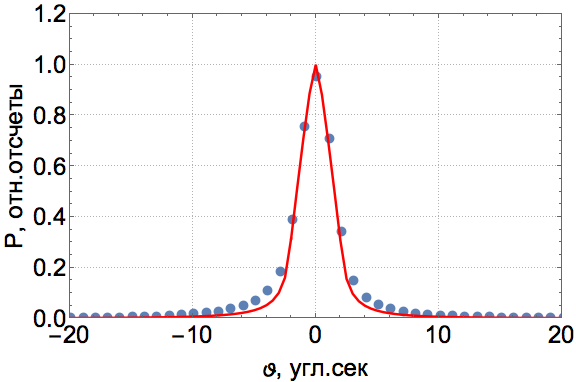
\includegraphics[width=0.45\textwidth]{images/non_disspers_20_40.png}\label{fig:f1}}
  \hfill
  \subfloat[$S_1 = 20 $ мкм; $ S_2 = 40$ мкм; ]{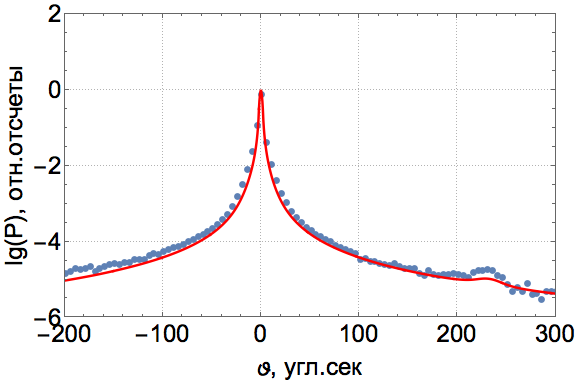
\includegraphics[width=0.45\textwidth]{images/non_disspers_20_40_log.png}\label{fig:non_disspers_kdo_1}}
  \hfill
  \subfloat[$S_1 = 300 $ мкм; $ S_2 = 200$ мкм;]{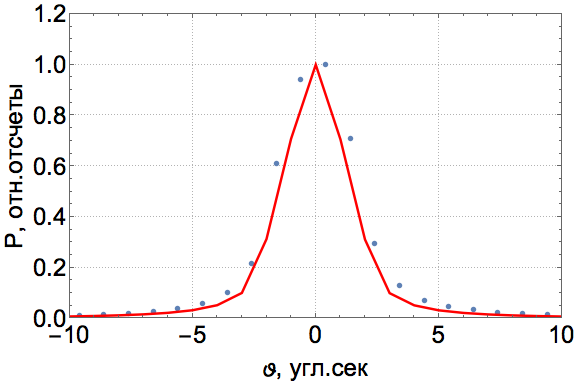
\includegraphics[width=0.45\textwidth]{images/non_disspers_300_200.png}\label{fig:f2}}
  \hfill
  \subfloat[$S_1 = 300 $ мкм; $ S_2 = 200$ мкм;]{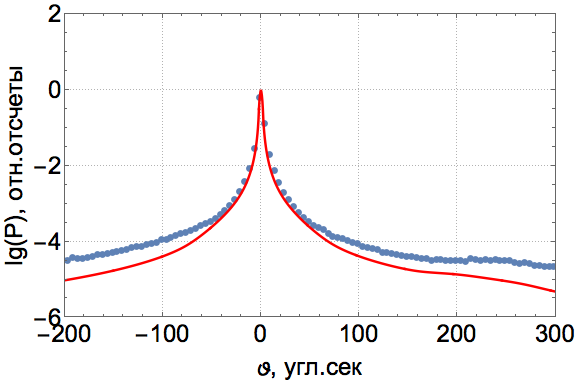
\includegraphics[width=0.45\textwidth]{images/non_disspers_300_200_log.png}\label{fig:f2}}
  \caption{Двухкристальная КДО для схемы с кристаллом монохроматором Si(220) и образцом  Si(220); $L_1= 570 $мм,
  $L_2 = 1005$ мм; $\delta = 0.1$ мм; (красная линия) - расчет, (синие точки) - эксперимент.}
  \label{ris:non_disspers_kdo}
\end{figure}

На рисунке \ref{fig:non_disspers_kdo_1} видно, что наряду с главным пиком, соответствующим $k_{\alpha1}$ лиинии
излучения, на которую настроен монохроматор, присутствует вклад от соседней характеристической линии
 $k_{\alpha2}$. Впервые, на это свойство двухкристальных КДО, получаемы в бездисперсионной
схеме, в случае использования рентгеновской трубки было указано авторами работы \cite{chuev2008}
